\section{Strumenti utilizzati}
\noindent Durante il mio percorso di sviluppo, ho avuto l'opportunità di utilizzare una serie di strumenti e tecnologie all'avanguardia (figura \ref*{fig:diagramma_strumenti}), che sono stati essenziali 
per facilitare vari aspetti del processo di sviluppo, dalla scrittura del codice alla gestione dei progetti. 
Per la documentazione, l'analisi dei requisiti e la progettazione delle basi di dati, ho utilizzato Confluence. 
Questo \textit{software} di collaborazione si è rivelato estremamente efficace nel creare, organizzare e condividere documenti di progetto.\\

\noindent Una volta completata l'analisi e creato le \textit{issues} su Jira, mi sono dedicato allo sviluppo del codice, 
utilizzando Intellij IDEA per il \textit{backend} e WebStorm per il \textit{frontend}. 
Questi due \gls{IDEg} hanno notevolmente semplificato il processo di sviluppo, migliorando sia la produttività che la qualità del codice prodotto.\\

\noindent Per la gestione del codice sorgente, ho scelto Git, un sistema di controllo versione distribuito, e Bitbucket, 
un servizio di \textit{hosting} per progetti Git, che insieme hanno fornito una soluzione robusta e affidabile. 
Inoltre, per la gestione dei \textit{database} a grafo, ho impiegato \textit{Neo4j Desktop}, un'applicazione che facilita la creazione, gestione e monitoraggio 
delle prestazioni dei \textit{database} Neo4j.\\

\noindent Il processo di compilazione e \textit{testing} è stato ottimizzato grazie all'uso di Gradle, un sistema di automazione che ha ridotto 
i tempi di rilascio migliorando la coerenza e l'affidabilità delle \textit{build}. Per il \textit{deployment}, ho utilizzato Docker, 
una piattaforma che ha rivoluzionato il nostro approccio, permettendo di impacchettare e distribuire applicazioni in ambienti isolati, assicurando 
coerenza tra gli ambienti di sviluppo, \textit{testing} e produzione.\\

\noindent Infine, per l'integrazione continua, ho scelto \textit{Jenkins}, uno strumento che ha automatizzato il ciclo di vita del \textit{software}, 
dalla \textit{build} al \textit{testing} fino al \textit{deployment}, aumentando la velocità di rilascio e riducendo la possibilità di errori. \\

\begin{figure}[!h] 
  \centering 
  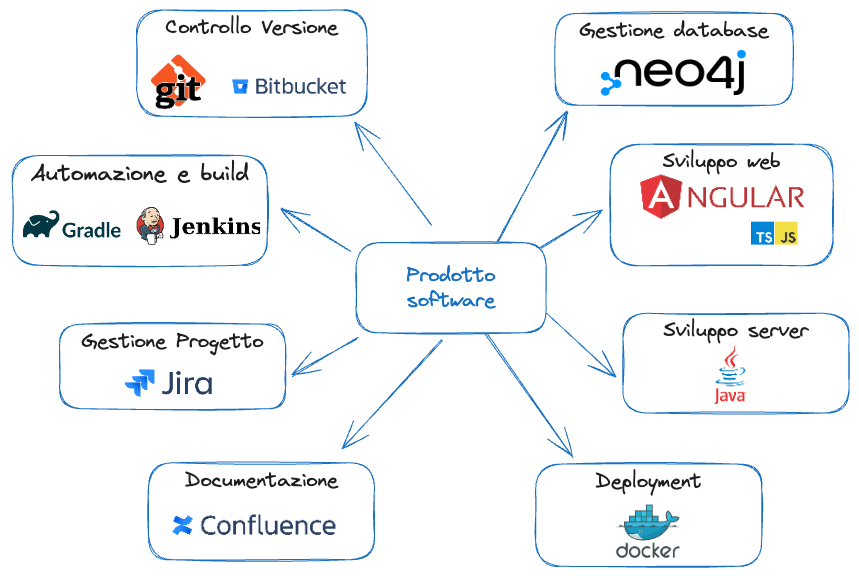
\includegraphics[width=1\columnwidth]{diagramma_strumenti} 
  \caption{Strumenti utilizzati}
  \label{fig:diagramma_strumenti}
\end{figure}

I linguaggi di programmazione utilizzati hanno incluso:

\begin{itemize}
\item \textbf{Java:} La mia principale lingua di programmazione, utilizzata per lo sviluppo di applicazioni robuste e ad alte prestazioni, sia \textit{web} che desktop;

\item \textbf{JavaScript:} Fondamentale per lo sviluppo \textit{frontend}  , ha permesso di creare interfacce utente interattive e dinamiche;

\item \textbf{TypeScript:} Utilizzato per aggiungere tipizzazione statica a JavaScript, migliorando la leggibilità e la manutenibilità del codice;

\item \textbf{Groovy:} Impiegato per script e automazioni, sfruttando la sua compatibilità con la \gls{JVM} e la sua sintassi espressiva;

\item \textbf{Cypher:} Il linguaggio di \textit{query} per Neo4j, essenziale per interrogare e manipolare i dati nei nostri \textit{database} a grafo.
\end{itemize}

Questi strumenti e linguaggi hanno formato il nucleo della mia cassetta degli attrezzi di sviluppo, permettendomi di affrontare una vasta gamma di sfide tecniche e di contribuire efficacemente 
ai progetti dell'azienda.

\subsection{Convenzioni}
Nel corso dello sviluppo dei progetti che impiegano il \textit{framework} interno, vengono adottate una serie di convenzioni standardizzate. 
Le convenzioni, archiviate in Confluence per un facile accesso da parte di tutti i dipendenti, 
sono state pensate per garantire coerenza, efficienza e qualità nel lavoro. Sono categorizzate come segue:

\begin{itemize}
\item \textbf{Documentazione:} Regole che stabiliscono come documentare efficacemente il codice sorgente. 
L'obiettivo è assicurare che ogni segmento di codice sia accompagnato da commenti chiari e concisi, che ne spieghino la funzione e la logica. 
Questo approccio, non solo facilita la comprensione del codice da parte di altri sviluppatori, ma è anche fondamentale per la manutenzione a lungo termine del \textit{software};

\item \textbf{Scrittura analisi:} Linee guida delineano il metodo per redigere analisi dei requisiti e progettazione delle strutture di basi di dati. 
L'obiettivo è garantire che le analisi siano scritte in modo chiaro e strutturato, facilitando la comprensione e la comunicazione tra i membri del \textit{team} e con i clienti;

\item \textbf{Progettazione:} Regole forniscono indicazioni su come progettare i componenti \textit{software}. 
L'enfasi è posta sulla creazione di \textit{design} modulari e riutilizzabili, che facilitano la manutenzione e l'estensione del codice nel tempo. 
Questo approccio aiuta a ridurre la complessità del codice e a migliorare la scalabilità delle applicazioni;

\item \textbf{Codifica:} Convenzioni che mirano a standardizzare lo stile di codifica. L'obiettivo è scrivere codice in modo uniforme, seguendo un insieme di regole che ne migliorino la leggibilità e la comprensione. Questo include convenzioni su nomi di variabili, strutture di controllo, formattazione del codice e commenti;

\item \textbf{Versionamento:} Regole stabiliscono come gestire il versionamento del codice sorgente. 
L'obiettivo è facilitare la tracciabilità delle modifiche e la gestione delle diverse versioni del \textit{software}. 
Questo è cruciale per il controllo qualità, la risoluzione dei \textit{bug} e la collaborazione tra i membri del \textit{team}.
\end{itemize}

Adottare convenzioni ha migliorato significativamente la qualità e l'efficienza del processo di sviluppo. Hanno fornito una base solida per la collaborazione e la standardizzazione, elementi chiave per il successo dei nostri progetti \textit{software}.
